\chapter{De celcyclus en de mitose}\label{ch:g11:cell-cycle-mitosis}

Plet de punt van een uienwortel onder een dekglaasje, kleur haar en kijk:
tussen honderden rustige \omterm{def:g10:cells-common-unit:cell}{cellen} met een ronde kern tonen er enkele iets
anders --- donkere X-vormige staafjes verzameld in het midden van de \omterm{def:g10:cells-common-unit:cell}{cel},
of twee groepen staafjes die naar de uiteinden uit elkaar worden
getrokken, of twee kleine kernen met een wand die zich ertussen vormt. Je
kijkt naar celdelingen die op verschillende momenten zijn betrapt, in een
weefsel dat een millimeter per dag groeit. Elk van die delingen geeft twee
volledige, gelijke stellen \omterm{def:g10:universal-dna:information}{chromosomen} aan twee dochtercellen. Dit
hoofdstuk volgt een \omterm{def:g10:cells-common-unit:cell}{cel} door één volledige cyclus, en kijkt van dichtbij
naar het uur waarin de \omterm{def:g10:universal-dna:information}{chromosomen} worden verdeeld.

\section{De celcyclus}

\begin{definition}[Celcyclus]\label{def:g11:cell-cycle-mitosis:cycle}
De \emph{celcyclus}\index{celcyclus} is de opeenvolging van
gebeurtenissen van de geboorte van een \omterm{def:g10:cells-common-unit:cell}{cel}, door deling, tot haar eigen
deling in tweeën. Zij omvat de \emph{interfase}, waarin de \omterm{def:g10:cells-common-unit:cell}{cel} groeit en
haar \omterm{def:g10:universal-dna:information}{DNA} kopieert, en de \emph{M-fase}, waarin eerst de kern zich deelt
(de \emph{mitose}\index{mitose}) en daarna het \omterm{def:g10:cells-common-unit:cell}{cytoplasma} (de
\emph{cytokinese}). De interfase bestaat uit drie delen: $\mathrm{G_1}$
(groei), S (\omterm{def:g11:dna-replication:replication}{DNA-replicatie}, \cref{ch:g11:dna-replication}) en
$\mathrm{G_2}$ (voorbereiding op de deling).
\end{definition}

\begin{omfigure}
\begin{tikzpicture}[font=\small]
  % pie: G1 11h, S 8h, G2 4h, M 1h  (24h) -> angles: G1 165°, S 120°, G2 60°, M 15°
  \fill[omDef!30] (0,0) -- (90:2.2) arc (90:-75:2.2) -- cycle;
  \fill[omProp!35] (0,0) -- (-75:2.2) arc (-75:-195:2.2) -- cycle;
  \fill[omMeth!35] (0,0) -- (-195:2.2) arc (-195:-255:2.2) -- cycle;
  \fill[omThm!50] (0,0) -- (-255:2.2) arc (-255:-270:2.2) -- cycle;
  \draw[thick] (0,0) circle (2.2);
  \foreach \a in {90,-75,-195,-255} \draw[thick] (0,0) -- (\a:2.2);
  \node at (10:1.3) {$\mathrm{G_1}$};
  \node at (-135:1.3) {S};
  \node at (-225:1.35) {$\mathrm{G_2}$};
  \node[anchor=south east] at (-262:2.35) {M};
  \node[anchor=west, align=left] at (2.6,1.3) {$\mathrm{G_1}$: groei, ongeveer \qty{11}{h}};
  \node[anchor=west, align=left] at (2.6,0.5) {S: DNA-replicatie, \qty{8}{h}};
  \node[anchor=west, align=left] at (2.6,-0.3) {$\mathrm{G_2}$: voorbereiding, \qty{4}{h}};
  \node[anchor=west, align=left] at (2.6,-1.1) {M: mitose en cytokinese, \qty{1}{h}};
  \draw[->, thick] (100:2.5) arc (100:130:2.5);
\end{tikzpicture}

{\small De \omterm{def:g11:cell-cycle-mitosis:cycle}{celcyclus} van een gewone delende menselijke \omterm{def:g10:cells-common-unit:cell}{cel}, ongeveer 24
uur. De interfase ($\mathrm{G_1}$, S, $\mathrm{G_2}$) neemt er 23 in
beslag, de deling zelf één. Veel \omterm{def:g10:cells-common-unit:cell}{cellen} verlaten de cyclus na
$\mathrm{G_1}$ en delen zich nooit meer.}
\end{omfigure}

\begin{proposition}[Het DNA door de cyclus heen]\label{prop:g11:cell-cycle-mitosis:dna}
Noem $q$ de hoeveelheid \omterm{def:g10:universal-dna:information}{DNA} in een \omterm{def:g10:cells-common-unit:organelle}{celkern} vlak na de deling. Zij blijft
$q$ gedurende $\mathrm{G_1}$, stijgt tijdens S gestaag naar $2q$ terwijl
de \omterm{def:g10:universal-dna:information}{chromosomen} worden gekopieerd, blijft $2q$ gedurende $\mathrm{G_2}$ en
het eerste deel van de \omterm{def:g11:cell-cycle-mitosis:cycle}{mitose}, en zakt aan het eind van de \omterm{def:g11:cell-cycle-mitosis:cycle}{mitose} in elke
dochterkern terug naar $q$. Het aantal \omterm{def:g10:universal-dna:information}{chromosomen} verandert tijdens S
niet: elk \omterm{def:g11:cell-cycle-mitosis:chromosome}{chromosoom} wordt gekopieerd tot twee gelijke
\emph{\omterm{def:g11:cell-cycle-mitosis:chromosome}{chromatiden}} die aan hun \emph{\omterm{def:g11:cell-cycle-mitosis:chromosome}{centromeer}} bijeen worden gehouden,
en splitst pas tijdens de \omterm{def:g11:cell-cycle-mitosis:cycle}{mitose} in twee \omterm{def:g10:universal-dna:information}{chromosomen}.
\end{proposition}
\admitted

\begin{omfigure}
\begin{tikzpicture}
\begin{axis}[
  width=0.9\linewidth, height=5.4cm,
  axis x line=bottom, axis y line=left,
  xmin=0, xmax=50, ymin=0, ymax=2.8,
  xlabel={tijd (h)}, ylabel={DNA per celkern},
  xlabel style={font=\small, at={(axis description cs:0.5,-0.1)}, anchor=north},
  ylabel style={font=\small},
  tick label style={font=\small}, xtick={0,11,19,23,24,35,43,47,48},
  xticklabels={0,11,19,23,,24,35,43,,48},
  ytick={1,2}, yticklabels={$q$, $2q$},
  clip=false,
]
\addplot[thick, omDef] coordinates {(0,1) (11,1) (19,2) (23,2) (23.9,2) (24,1) (35,1) (43,2) (47,2) (47.9,2) (48,1) (50,1)};
\node[font=\small, anchor=south] at (axis cs:5.5,2.25) {$\mathrm{G_1}$};
\node[font=\small, anchor=south] at (axis cs:15,2.25) {S};
\node[font=\small, anchor=south] at (axis cs:21,2.25) {$\mathrm{G_2}$};
\node[font=\small, anchor=south] at (axis cs:29.5,2.25) {$\mathrm{G_1}$};
\node[font=\small, anchor=south] at (axis cs:39,2.25) {S};
\node[font=\small, anchor=south] at (axis cs:45,2.25) {$\mathrm{G_2}$};
\node[font=\small, anchor=south, omThm] at (axis cs:23.5,2.55) {M};
\node[font=\small, anchor=south, omThm] at (axis cs:47.5,2.55) {M};
\draw[dashed, gray] (axis cs:11,0) -- (axis cs:11,2.2);
\draw[dashed, gray] (axis cs:19,0) -- (axis cs:19,2.2);
\draw[dashed, gray] (axis cs:23,0) -- (axis cs:23,2.2);
\draw[dashed, gray] (axis cs:24,0) -- (axis cs:24,2.2);
\draw[dashed, gray] (axis cs:35,0) -- (axis cs:35,2.2);
\draw[dashed, gray] (axis cs:43,0) -- (axis cs:43,2.2);
\draw[dashed, gray] (axis cs:47,0) -- (axis cs:47,2.2);
\end{axis}
\end{tikzpicture}

{\small Hoeveelheid \omterm{def:g10:universal-dna:information}{DNA} in één \omterm{def:g10:cells-common-unit:organelle}{celkern} over twee opeenvolgende cycli van
24 uur. Zij verdubbelt tijdens S en halveert aan het eind van de \omterm{def:g11:cell-cycle-mitosis:cycle}{mitose};
een dochtercel begint altijd met $q$.}
\end{omfigure}

\begin{example}[De kromme lezen]\label{ex:g11:cell-cycle-mitosis:reading}
Een \omterm{def:g10:cells-common-unit:cell}{cel} die op $2q$ wordt gemeten, kan in $\mathrm{G_2}$ of in het begin
van de \omterm{def:g11:cell-cycle-mitosis:cycle}{mitose} zijn; op $1.5q$ is zij zeker in S, halverwege de
replicatie; op $q$ is zij in $\mathrm{G_1}$ --- of zij heeft de cyclus
voorgoed verlaten, zoals een zenuwcel of een \omterm{def:g10:muscles-and-joints:muscle}{spiervezel}, die hun leven
lang op $q$ blijven. Een weefsel waarin elke \omterm{def:g10:cells-common-unit:cell}{cel} op $q$ staat, is een
weefsel dat is opgehouden met delen.
\end{example}

\section{Chromosomen, in beeld}

\begin{definition}[Chromosoom, chromatide, karyotype]\label{def:g11:cell-cycle-mitosis:chromosome}
Een \emph{chromosoom} is één DNA-molecuul met zijn verpakkingseiwitten.
Tussen twee delingen is het een losse, onzichtbare draad; aan het begin
van de \omterm{def:g11:cell-cycle-mitosis:cycle}{mitose} rolt het zich op tot een compact staafje dat onder de
lichtmicroscoop zichtbaar is. Na de replicatie bestaat elk chromosoom uit
twee gelijke \emph{chromatiden}\index{chromatide}, verbonden bij het
\emph{centromeer}\index{centromeer}: de vertrouwde X-vorm. Het
\emph{karyotype}\index{karyotype} van een \omterm{def:g10:biodiversity-scales:species}{soort} is haar volledige stel
\omterm{def:g10:universal-dna:information}{chromosomen}, in de metafase gefotografeerd en op grootte in paren
gerangschikt: een menselijke \omterm{def:g10:cells-common-unit:cell}{cel} heeft er 46, in 23 paren, waarbij de
leden van een paar \emph{\omterm{def:g10:common-ancestry:homology}{homoloog}} zijn --- dezelfde \omterm{def:g10:universal-dna:gene}{genen} op dezelfde
plaatsen, één van elke ouder.
\end{definition}

\begin{omfigure}
\begin{tikzpicture}[font=\scriptsize, line cap=round]
  % 22 autosome pairs of decreasing size, then X and Y; each chromosome = two chromatids
  \tikzset{chrom/.style={line width=2.6pt, omDef!75}}
  \foreach \n/\h/\c in {1/2.4/0.55, 2/2.3/0.5, 3/2.0/0.5, 4/1.9/0.35, 5/1.8/0.35, 6/1.7/0.45, 7/1.55/0.42, 8/1.45/0.4}
    { \pgfmathsetmacro{\x}{(\n-1)*1.55}
      \draw[chrom] (\x,0) -- (\x,\h); \draw[chrom] (\x+0.22,0) -- (\x+0.22,\h);
      \fill[omThm] (\x+0.11,{\h*\c}) circle (2pt);
      \node[anchor=north] at (\x+0.11,-0.08) {\n}; }
  \foreach \n/\h/\c in {9/1.4/0.35, 10/1.35/0.35, 11/1.35/0.4, 12/1.3/0.3, 13/1.1/0.15, 14/1.05/0.15, 15/1.0/0.15, 16/0.9/0.45}
    { \pgfmathsetmacro{\x}{(\n-9)*1.55}
      \draw[chrom] (\x,-3.2) -- (\x,-3.2+\h); \draw[chrom] (\x+0.22,-3.2) -- (\x+0.22,-3.2+\h);
      \fill[omThm] (\x+0.11,{-3.2+\h*\c}) circle (2pt);
      \node[anchor=north] at (\x+0.11,-3.28) {\n}; }
  \foreach \n/\h/\c in {17/0.85/0.3, 18/0.8/0.2, 19/0.65/0.5, 20/0.65/0.5, 21/0.5/0.2, 22/0.5/0.2}
    { \pgfmathsetmacro{\x}{(\n-17)*1.55}
      \draw[chrom] (\x,-5.6) -- (\x,-5.6+\h); \draw[chrom] (\x+0.22,-5.6) -- (\x+0.22,-5.6+\h);
      \fill[omThm] (\x+0.11,{-5.6+\h*\c}) circle (2pt);
      \node[anchor=north] at (\x+0.11,-5.68) {\n}; }
  % sex chromosomes
  \draw[chrom] (9.3,-5.6) -- (9.3,-4.1); \draw[chrom] (9.52,-5.6) -- (9.52,-4.1); \fill[omThm] (9.41,-4.85) circle (2pt);
  \node[anchor=north] at (9.41,-5.68) {X};
  \draw[chrom] (10.85,-5.6) -- (10.85,-5.1); \draw[chrom] (11.07,-5.6) -- (11.07,-5.1); \fill[omThm] (10.96,-5.5) circle (2pt);
  \node[anchor=north] at (10.96,-5.68) {Y};
\end{tikzpicture}

{\small Een menselijk \omterm{def:g11:cell-cycle-mitosis:chromosome}{karyotype}, schematisch: de 22 paren gewone
\omterm{def:g10:universal-dna:information}{chromosomen} genummerd op afnemende grootte, en daarna de
geslachtschromosomen --- hier X en Y, dus een man. Elk \omterm{def:g11:cell-cycle-mitosis:chromosome}{chromosoom} is als
zijn twee \omterm{def:g11:cell-cycle-mitosis:chromosome}{chromatiden} getekend, met het \omterm{def:g11:cell-cycle-mitosis:chromosome}{centromeer} in rood.}
\end{omfigure}

\begin{omfigure}
\begin{tikzpicture}[font=\small, line cap=round]
  % single chromatid chromosome
  \draw[line width=5pt, omDef!70] (0,-1.2) -- (0,1.2);
  \fill[omThm] (0,0.2) circle (3.5pt);
  \node[anchor=north, align=center] at (0,-1.5) {vóór de S-fase:\\ één chromatide};
  % arrow
  \draw[->, thick] (1.2,0) -- (2.6,0) node[midway, above] {S};
  % two chromatid chromosome
  \draw[line width=5pt, omDef!70] (3.6,-1.2) .. controls (3.75,-0.3) and (3.75,0.3) .. (3.6,1.2);
  \draw[line width=5pt, omDef!70] (4.2,-1.2) .. controls (4.05,-0.3) and (4.05,0.3) .. (4.2,1.2);
  \fill[omThm] (3.9,0.2) circle (3.5pt);
  \node[anchor=north, align=center] at (3.9,-1.5) {na de S-fase:\\ twee gelijke chromatiden};
  \draw[->] (5.6,0.2) -- (4.15,0.2) node[pos=0, anchor=west] {centromeer};
  \draw[->] (5.6,0.9) -- (4.35,0.9) node[pos=0, anchor=west] {chromatide};
  % after anaphase
  \draw[->, thick] (8.6,0) -- (10.0,0) node[midway, above] {anafase};
  \draw[line width=5pt, omDef!70] (10.8,-1.2) -- (10.8,1.2);
  \fill[omThm] (10.8,0.2) circle (3.5pt);
  \draw[line width=5pt, omDef!70] (11.8,-1.2) -- (11.8,1.2);
  \fill[omThm] (11.8,0.2) circle (3.5pt);
  \node[anchor=north, align=center] at (11.3,-1.5) {twee chromosomen,\\ één voor elke cel};
\end{tikzpicture}

{\small Eén \omterm{def:g11:cell-cycle-mitosis:chromosome}{chromosoom} door de cyclus heen. De replicatie maakt er twee
\omterm{def:g11:cell-cycle-mitosis:chromosome}{chromatiden} van, verbonden bij het \omterm{def:g11:cell-cycle-mitosis:chromosome}{centromeer}; de anafase scheidt hen in
twee \omterm{def:g10:universal-dna:information}{chromosomen} met één \omterm{def:g11:cell-cycle-mitosis:chromosome}{chromatide}, één voor elke dochtercel. Het aantal
\omterm{def:g10:universal-dna:information}{chromosomen} verandert alleen in de anafase.}
\end{omfigure}

\section{De mitose, stap voor stap}

\begin{proposition}[De vier stadia van de mitose]\label{prop:g11:cell-cycle-mitosis:stages}
De \omterm{def:g11:cell-cycle-mitosis:cycle}{mitose} is een doorlopende beweging, die in vier stadia wordt
beschreven.
\begin{enumerate}
  \item \emph{Profase}: de \omterm{def:g10:universal-dna:information}{chromosomen} verdichten zich tot zichtbare
        staafjes met twee \omterm{def:g11:cell-cycle-mitosis:chromosome}{chromatiden}; het kernmembraan valt uiteen; er
        vormt zich een \emph{spoel} van eiwitvezels tussen de twee polen
        van de \omterm{def:g10:cells-common-unit:cell}{cel}.
  \item \emph{Metafase}: de \omterm{def:g10:universal-dna:information}{chromosomen}, met hun \omterm{def:g11:cell-cycle-mitosis:chromosome}{centromeer} aan
        spoelvezels gehecht, gaan op het evenaarsvlak van de \omterm{def:g10:cells-common-unit:cell}{cel} in het
        gelid staan.
  \item \emph{Anafase}: de \omterm{def:g11:cell-cycle-mitosis:chromosome}{centromeren} splitsen; de twee \omterm{def:g11:cell-cycle-mitosis:chromosome}{chromatiden} van
        elk \omterm{def:g11:cell-cycle-mitosis:chromosome}{chromosoom}, nu twee \omterm{def:g10:universal-dna:information}{chromosomen}, worden door de korter
        wordende vezels naar tegenovergestelde polen getrokken.
  \item \emph{Telofase}: rond elk stel vormt zich weer een kernmembraan;
        de \omterm{def:g10:universal-dna:information}{chromosomen} rollen zich af. De cytokinese verdeelt daarna het
        \omterm{def:g10:cells-common-unit:cell}{cytoplasma} --- door insnoering bij dierlijke \omterm{def:g10:cells-common-unit:cell}{cellen}, door een
        nieuwe wand te bouwen bij plantencellen.
\end{enumerate}
Elke dochtercel ontvangt één \omterm{def:g11:cell-cycle-mitosis:chromosome}{chromatide} van elk \omterm{def:g11:cell-cycle-mitosis:chromosome}{chromosoom}: evenveel
\omterm{def:g10:universal-dna:information}{chromosomen} als de moeder, met hetzelfde \omterm{def:g10:universal-dna:information}{DNA}.
\end{proposition}
\admitted

\begin{omfigure}
\begin{tikzpicture}[font=\small, line cap=round]
  \tikzset{cellb/.style={draw, thick, fill=omDef!5, rounded corners=10pt, minimum width=2.9cm, minimum height=2.6cm},
           chr/.style={line width=3pt, omDef!80}, cen/.style={fill=omThm}}
  % prophase
  \begin{scope}
    \node[cellb] at (0,0) {};
    \draw[thick, dashed, gray] (0,0) circle (0.95);
    \draw[chr] (-0.5,0.5) .. controls (-0.35,0.1) .. (-0.5,-0.3); \draw[chr] (-0.2,0.5) .. controls (-0.35,0.1) .. (-0.2,-0.3); \fill[cen] (-0.35,0.1) circle (2pt);
    \draw[chr] (0.2,0.6) .. controls (0.35,0.2) .. (0.2,-0.2); \draw[chr] (0.5,0.6) .. controls (0.35,0.2) .. (0.5,-0.2); \fill[cen] (0.35,0.2) circle (2pt);
    \node[anchor=north, align=center] at (0,-1.45) {profase};
  \end{scope}
  % metaphase
  \begin{scope}[xshift=3.6cm]
    \node[cellb] at (0,0) {};
    \fill (0,1.1) circle (2pt); \fill (0,-1.1) circle (2pt);
    \foreach \x in {-0.45,0.45} { \draw[gray] (0,1.1) -- (\x,0.05); \draw[gray] (0,-1.1) -- (\x,-0.05); }
    \foreach \x in {-0.45,0.45} {
      \draw[chr] (\x-0.13,0.55) .. controls (\x,0.0) .. (\x-0.13,-0.55);
      \draw[chr] (\x+0.13,0.55) .. controls (\x,0.0) .. (\x+0.13,-0.55);
      \fill[cen] (\x,0) circle (2pt);
    }
    \draw[dashed, gray] (-1.3,0) -- (1.3,0);
    \node[anchor=north, align=center] at (0,-1.45) {metafase};
  \end{scope}
  % anaphase
  \begin{scope}[xshift=7.2cm]
    \node[cellb] at (0,0) {};
    \fill (0,1.1) circle (2pt); \fill (0,-1.1) circle (2pt);
    \foreach \x in {-0.45,0.45} { \draw[gray] (0,1.1) -- (\x,0.6); \draw[gray] (0,-1.1) -- (\x,-0.6); }
    \foreach \x in {-0.45,0.45} {
      \draw[chr] (\x,0.6) .. controls (\x-0.1,0.4) .. (\x-0.25,0.05);
      \draw[chr] (\x,0.6) .. controls (\x+0.1,0.4) .. (\x+0.25,0.05);
      \fill[cen] (\x,0.6) circle (2pt);
      \draw[chr] (\x,-0.6) .. controls (\x-0.1,-0.4) .. (\x-0.25,-0.05);
      \draw[chr] (\x,-0.6) .. controls (\x+0.1,-0.4) .. (\x+0.25,-0.05);
      \fill[cen] (\x,-0.6) circle (2pt);
    }
    \node[anchor=north, align=center] at (0,-1.45) {anafase};
  \end{scope}
  % telophase
  \begin{scope}[xshift=10.8cm]
    \draw[thick, fill=omDef!5] (-1.45,1.3) .. controls (-1.6,0.3) and (-0.3,0.3) .. (0,0) .. controls (-0.3,-0.3) and (-1.6,-0.3) .. (-1.45,-1.3) -- cycle;
    \draw[thick, fill=omDef!5] (1.45,1.3) .. controls (1.6,0.3) and (0.3,0.3) .. (0,0) .. controls (0.3,-0.3) and (1.6,-0.3) .. (1.45,-1.3) -- cycle;
    \draw[thick, fill=omDef!5, rounded corners=10pt] (-1.45,-1.3) rectangle (1.45,1.3);
    \draw[thick, fill=white] (-1.45,1.3) .. controls (-1.6,0.3) and (-0.3,0.3) .. (0,0) .. controls (-0.3,-0.3) and (-1.6,-0.3) .. (-1.45,-1.3);
    \draw[thick, fill=white] (1.45,1.3) .. controls (1.6,0.3) and (0.3,0.3) .. (0,0) .. controls (0.3,-0.3) and (1.6,-0.3) .. (1.45,-1.3);
    \draw[thick, dashed, gray] (-0.75,0) circle (0.5); \draw[thick, dashed, gray] (0.75,0) circle (0.5);
    \foreach \x in {-0.9,-0.6,0.6,0.9} \draw[chr] (\x,0.25) -- (\x,-0.25);
    \node[anchor=north, align=center] at (0,-1.45) {telofase en\\ cytokinese};
  \end{scope}
\end{tikzpicture}

{\small \omterm{def:g11:cell-cycle-mitosis:cycle}{Mitose} van een \omterm{def:g10:cells-common-unit:cell}{cel} met twee \omterm{def:g10:universal-dna:information}{chromosomen} ($2n = 2$), elk al uit
twee \omterm{def:g11:cell-cycle-mitosis:chromosome}{chromatiden} opgebouwd. Profase: verdichting, kernmembraan
verdwenen. Metafase: opstelling op de evenaar, \omterm{def:g11:cell-cycle-mitosis:chromosome}{centromeren} aan de spoel
gehecht. Anafase: \omterm{def:g11:cell-cycle-mitosis:chromosome}{chromatiden} naar de polen uit elkaar getrokken.
Telofase: twee kernen vormen zich opnieuw en de \omterm{def:g10:cells-common-unit:cell}{cel} deelt zich.}
\end{omfigure}

\begin{omfigure}
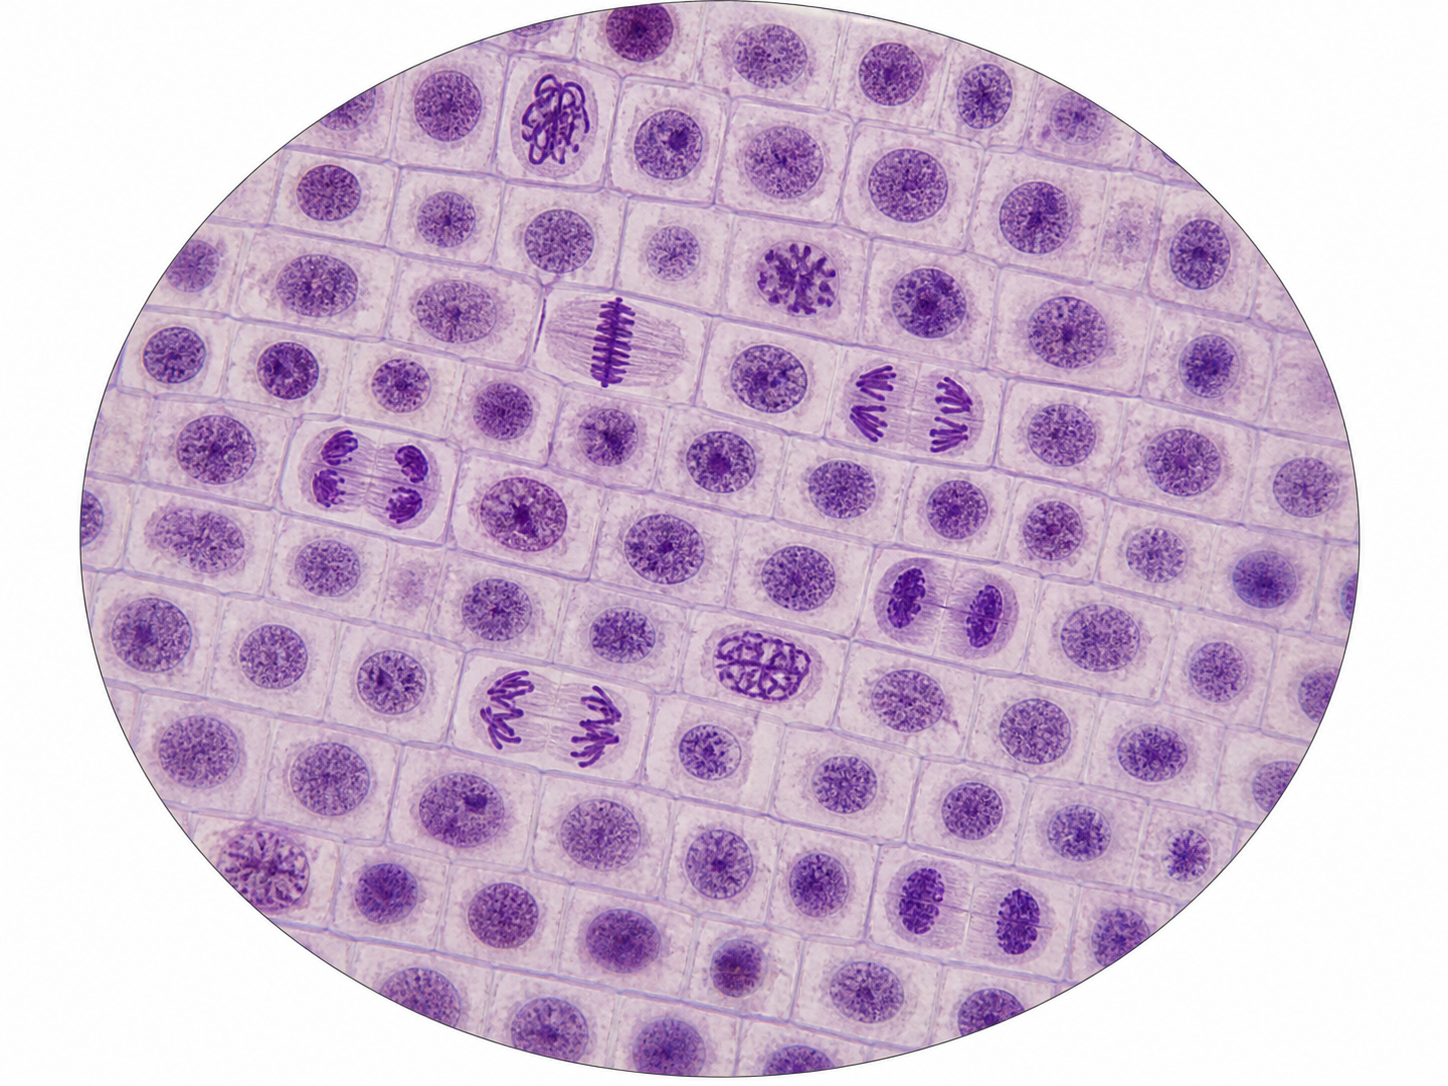
\includegraphics[width=0.58\linewidth]{images/book2/ai/g11-mitosis-root-tip.png}

{\small Een geplette uienwortelpunt onder de lichtmicroscoop. De meeste
\omterm{def:g10:cells-common-unit:cell}{cellen} zijn in interfase; enkele tonen verdichte \omterm{def:g10:universal-dna:information}{chromosomen} in
verschillende stadia van de \omterm{def:g11:cell-cycle-mitosis:cycle}{mitose}. Tellen welk deel in elk stadium is,
meet hoelang elk stadium duurt.}
\end{omfigure}

\begin{example}[Tellen in de wortelpunt]\label{ex:g11:cell-cycle-mitosis:count}
Van 600 getelde \omterm{def:g10:cells-common-unit:cell}{cellen} in een wortelpunt zijn er 540 in interfase en 60
in \omterm{def:g11:cell-cycle-mitosis:cycle}{mitose}: een \emph{mitose-index} van 10\%. Duurt de cyclus 20 uur, dan
duurt de \omterm{def:g11:cell-cycle-mitosis:cycle}{mitose} ongeveer $0.10 \times 20 = \qty{2}{h}$; en zijn 36 van de
60 delende \omterm{def:g10:cells-common-unit:cell}{cellen} in profase, dan neemt de profase $36/60$ van die twee
uur in beslag, zo'n 72 minuten, terwijl de anafase, in slechts 4 \omterm{def:g10:cells-common-unit:cell}{cellen}
gezien, ongeveer 8 minuten duurt. Het zeldzaamste stadium is het snelste.
\end{example}

\begin{method}[Chromosomen en chromatiden tellen]\label{met:g11:cell-cycle-mitosis:counting}
Voor een \omterm{def:g10:biodiversity-scales:species}{soort} met $2n$ \omterm{def:g10:universal-dna:information}{chromosomen}:
\begin{enumerate}
  \item in $\mathrm{G_1}$: $2n$ \omterm{def:g10:universal-dna:information}{chromosomen} met elk één \omterm{def:g11:cell-cycle-mitosis:chromosome}{chromatide}, \omterm{def:g10:universal-dna:information}{DNA}
        $q$;
  \item na S, gedurende $\mathrm{G_2}$, profase en metafase: $2n$
        \omterm{def:g10:universal-dna:information}{chromosomen} met elk twee \omterm{def:g11:cell-cycle-mitosis:chromosome}{chromatiden} ($4n$ \omterm{def:g11:cell-cycle-mitosis:chromosome}{chromatiden}), \omterm{def:g10:universal-dna:information}{DNA}
        $2q$;
  \item vanaf de anafase: $4n$ \omterm{def:g10:universal-dna:information}{chromosomen} met één \omterm{def:g11:cell-cycle-mitosis:chromosome}{chromatide} in de \omterm{def:g10:cells-common-unit:cell}{cel},
        waarvan $2n$ naar elke pool gaan;
  \item in elke dochtercel: $2n$ \omterm{def:g10:universal-dna:information}{chromosomen} met elk één \omterm{def:g11:cell-cycle-mitosis:chromosome}{chromatide}, \omterm{def:g10:universal-dna:information}{DNA}
        $q$.
\end{enumerate}
Een \omterm{def:g11:cell-cycle-mitosis:chromosome}{chromatide} wordt een \omterm{def:g11:cell-cycle-mitosis:chromosome}{chromosoom} op het moment dat haar \omterm{def:g11:cell-cycle-mitosis:chromosome}{centromeer}
splitst.
\end{method}

\begin{example}[Menselijke getallen]\label{ex:g11:cell-cycle-mitosis:human}
Een menselijke \omterm{def:g10:cells-common-unit:cell}{cel} in metafase bevat 46 \omterm{def:g10:universal-dna:information}{chromosomen} en 92 \omterm{def:g11:cell-cycle-mitosis:chromosome}{chromatiden}; in
anafase 92 \omterm{def:g10:universal-dna:information}{chromosomen}, waarvan er 46 naar elke pool gaan; elke dochter
46 \omterm{def:g10:universal-dna:information}{chromosomen} met elk één \omterm{def:g11:cell-cycle-mitosis:chromosome}{chromatide}, en precies het \omterm{def:g10:universal-dna:information}{DNA} dat de moeder
aan het begin van haar cyclus had.
\end{example}

\section{Waar de mitose voor dient}

\begin{proposition}[Gelijkheid en waar zij toe dient]\label{prop:g11:cell-cycle-mitosis:conformity}
Doordat de replicatie getrouw is en de \omterm{def:g11:cell-cycle-mitosis:cycle}{mitose} de \omterm{def:g11:cell-cycle-mitosis:chromosome}{chromatiden} precies
verdeelt, draagt elke \omterm{def:g10:cells-common-unit:cell}{cel} van een meercellig lichaam dezelfde \omterm{def:g10:universal-dna:information}{genetische
informatie} als de bevruchte eicel waarvan zij afstamt. De \omterm{def:g11:cell-cycle-mitosis:cycle}{mitose} is het
mechanisme van de groei (het embryo, de wortelpunt), van de vernieuwing
(huid, darmbekleding, bloed: alleen al het beenmerg maakt zo'n
$\num{2e11}$ \omterm{def:g10:cells-common-unit:cell}{cellen} per dag) en van het herstel (het genezen van wonden);
bij eencellige eukaryoten is zij de voortplanting zelf. Haar regeling ---
het besluit om de cyclus in te gaan, de controles vóór S en vóór de
anafase --- is het onderwerp van \cref{ch:g11:cancer}.
\end{proposition}
\admitted

\begin{remark}[Niet alles deelt zich]\label{rem:g11:cell-cycle-mitosis:notall}
De meeste zenuwcellen en hartspiercellen verlaten de cyclus in de vroege
kindertijd en komen er nooit meer in: schade aan hen wordt niet door
deling hersteld, en daarom laten een ruggenmergletsel of een hartinfarct
blijvend verlies achter. Levercellen rusten maandenlang in
$\mathrm{G_1}$, maar gaan de cyclus weer in wanneer een deel van de lever
wordt weggenomen, en laten het orgaan binnen weken weer aangroeien. Welke
\omterm{def:g10:cells-common-unit:cell}{cellen} zich mogen delen, en wanneer, is een van de strengste regelingen
van het lichaam.
\end{remark}

\section{Oefeningen}

\begin{exercise}[$\star$]\label{exo:g11:cell-cycle-mitosis:1}
Noem de vier fasen van de \omterm{def:g11:cell-cycle-mitosis:cycle}{celcyclus} en zeg wat er in elk gebeurt.
\end{exercise}

\begin{exercise}[$\star$]\label{exo:g11:cell-cycle-mitosis:2}
Definieer \omterm{def:g11:cell-cycle-mitosis:chromosome}{chromatide} en \omterm{def:g11:cell-cycle-mitosis:chromosome}{centromeer}. Wanneer heeft een \omterm{def:g11:cell-cycle-mitosis:chromosome}{chromosoom} twee
\omterm{def:g11:cell-cycle-mitosis:chromosome}{chromatiden}?
\end{exercise}

\begin{exercise}[$\star$]\label{exo:g11:cell-cycle-mitosis:3}
Noem de vier stadia van de \omterm{def:g11:cell-cycle-mitosis:cycle}{mitose} met van elk één sleutelgebeurtenis.
\end{exercise}

\begin{exercise}[$\star$]\label{exo:g11:cell-cycle-mitosis:4}
Een \omterm{def:g10:cells-common-unit:organelle}{celkern} bevat $1.5q$ \omterm{def:g10:universal-dna:information}{DNA}. In welke fase is de \omterm{def:g10:cells-common-unit:cell}{cel}?
\end{exercise}

\begin{exercise}[$\star$]\label{exo:g11:cell-cycle-mitosis:5}
Hoeveel \omterm{def:g10:universal-dna:information}{chromosomen}, en hoeveel \omterm{def:g11:cell-cycle-mitosis:chromosome}{chromatiden}, heeft een menselijke \omterm{def:g10:cells-common-unit:cell}{cel} in
$\mathrm{G_2}$?
\end{exercise}

\begin{exercise}[$\star\star$]\label{exo:g11:cell-cycle-mitosis:6}
Geef uit de figuur van de DNA-hoeveelheid de duur van elke fase en zeg in
welke fasen een \omterm{def:g10:cells-common-unit:cell}{cel} met $2q$ te vinden is.
\end{exercise}

\begin{exercise}[$\star\star$]\label{exo:g11:cell-cycle-mitosis:7}
Een muis heeft $2n = 40$. Geef het aantal \omterm{def:g10:universal-dna:information}{chromosomen} en \omterm{def:g11:cell-cycle-mitosis:chromosome}{chromatiden} in
een \omterm{def:g10:cells-common-unit:cell}{cel} in metafase, in anafase (de hele \omterm{def:g10:cells-common-unit:cell}{cel}), en in een dochtercel.
\end{exercise}

\begin{exercise}[$\star\star$]\label{exo:g11:cell-cycle-mitosis:8}
In een wortelpunt worden 800 \omterm{def:g10:cells-common-unit:cell}{cellen} geteld: 720 in interfase, 48 in
profase, 16 in metafase, 6 in anafase, 10 in telofase. Bereken de
mitose-index en, voor een cyclus van 24 uur, de duur van elk stadium.
\end{exercise}

\begin{exercise}[$\star\star$]\label{exo:g11:cell-cycle-mitosis:9}
Colchicine, een stof uit herfsttijlozen, verhindert dat de spoel zich
vormt. Voorspel wat er met een delende \omterm{def:g10:cells-common-unit:cell}{cel} gebeurt die ermee wordt
behandeld, en waarom biologen haar gebruiken om \omterm{def:g11:cell-cycle-mitosis:chromosome}{karyotypes} te maken.
\end{exercise}

\begin{exercise}[$\star\star$]\label{exo:g11:cell-cycle-mitosis:10}
Leg uit waarom de \omterm{def:g10:universal-dna:information}{chromosomen} zich moeten verdichten voordat zij worden
verplaatst, en waarom zij zich daarna weer afrollen.
\end{exercise}

\begin{exercise}[$\star\star$]\label{exo:g11:cell-cycle-mitosis:11}
Een bevruchte eicel deelt zich in de eerste dagen om de 12 uur. Hoeveel
\omterm{def:g10:cells-common-unit:cell}{cellen} zijn er na 5 dagen? Zou elke deling een volledige $\mathrm{G_1}$
nodig hebben?
\end{exercise}

\begin{exercise}[$\star\star\star$]\label{exo:g11:cell-cycle-mitosis:12}
In de anafase gaan de twee \omterm{def:g11:cell-cycle-mitosis:chromosome}{chromatiden} van één \omterm{def:g11:cell-cycle-mitosis:chromosome}{chromosoom} niet uiteen en
belanden zij allebei bij dezelfde pool. Beschrijf de twee dochtercellen
(aantal \omterm{def:g10:universal-dna:information}{chromosomen}, \omterm{def:g10:universal-dna:information}{DNA}) en leg uit waarom zo'n fout in een lichaamscel
meestal zonder gevolg blijft, maar in sommige gevallen ernstig is.
\end{exercise}

\begin{exercise}[$\star\star\star$]\label{exo:g11:cell-cycle-mitosis:13}
Het beenmerg maakt $\num{2e11}$ bloedcellen per dag. Schat, als een
voorlopercel in het merg een cyclus van 24 uur heeft, hoeveel
voorlopercellen zich op enig moment delen, en becommentarieer wat een
middel dat de \omterm{def:g11:cell-cycle-mitosis:cycle}{mitose} blokkeert binnen een week met het bloed zou doen.
\end{exercise}

\begin{exercise}[$\star\star\star$]\label{exo:g11:cell-cycle-mitosis:14}
Leg uit waarom een \omterm{def:g11:cell-cycle-mitosis:chromosome}{karyotype} wordt gemaakt van \omterm{def:g10:cells-common-unit:cell}{cellen} die in de metafase
zijn stilgezet, en niet in de interfase of de anafase.
\end{exercise}

\begin{exercise}[$\star\star\star$]\label{exo:g11:cell-cycle-mitosis:15}
Van een lever wordt twee derde weggenomen; binnen drie weken is hij weer
aangegroeid. Beschrijf met de \omterm{def:g11:cell-cycle-mitosis:cycle}{celcyclus} wat zijn \omterm{def:g10:cells-common-unit:cell}{cellen} deden, en zeg hoe
het DNA-gehalte van de levercellen op dag 3 eruitzag vergeleken met dag 0.
\end{exercise}

\section{Probleem: Het uurrooster van een wortelpunt}

\begin{problem}[{Weekendprobleem --- een wortelpunt cel voor cel geteld:
de duur van elk stadium van de cyclus, het DNA op elk moment, de cellen
die een wortel op een dag maakt, en de acht minuten van de anafase}]
\label{pb:g11:cell-cycle-mitosis:1}
Een klas plet en kleurt de punt van een knoflookwortel ($2n = 16$) en
telt 1000 \omterm{def:g10:cells-common-unit:cell}{cellen} in de groeizone: 900 in interfase, 60 in profase, 18 in
metafase, 8 in anafase, 14 in telofase. Onafhankelijke metingen geven de
cyclus van deze \omterm{def:g10:cells-common-unit:cell}{cellen} als 20 uur. Neem aan dat de groeizone
20\,000 \omterm{def:g10:cells-common-unit:cell}{cellen} bevat.

\medskip
\noindent\textbf{Deel I --- De mitose-index.}
\begin{enumerate}
  \item Bereken de mitose-index van het weefsel.
  \item Bereken de duur van de \omterm{def:g11:cell-cycle-mitosis:cycle}{mitose}, aangenomen dat het deel van de
        \omterm{def:g10:cells-common-unit:cell}{cellen} in een stadium gelijk is aan het deel van de cyclus dat
        daarin wordt doorgebracht.
  \item Bereken de duur van elk van de vier stadia.
  \item Welk stadium is het kortste? Stel voor waarom het zo snel kan
        gaan.
  \item Waarom vergt de methode dat er veel \omterm{def:g10:cells-common-unit:cell}{cellen} worden geteld, en
        waarom moeten die alleen uit de groeizone komen?
\end{enumerate}

\medskip
\noindent\textbf{Deel II --- \omterm{def:g10:universal-dna:information}{Chromosomen} en \omterm{def:g10:universal-dna:information}{DNA}.}
\begin{enumerate}[resume]
  \item Hoeveel \omterm{def:g10:universal-dna:information}{chromosomen}, en hoeveel \omterm{def:g11:cell-cycle-mitosis:chromosome}{chromatiden}, bevat een
        knoflookcel in de metafase?
  \item Hoeveel \omterm{def:g10:universal-dna:information}{chromosomen} bewegen er in een \omterm{def:g10:cells-common-unit:cell}{cel} in anafase, en hoeveel
        bereiken elke pool?
  \item Noem $q$ het \omterm{def:g10:universal-dna:information}{DNA} van een dochtercel en geef het DNA-gehalte van
        een \omterm{def:g10:cells-common-unit:cell}{cel} in profase, in anafase (de hele \omterm{def:g10:cells-common-unit:cell}{cel}) en in telofase (elke
        kern).
  \item Hoeveel van de 900 \omterm{def:g10:cells-common-unit:cell}{cellen} in interfase zijn er ruwweg in S, als
        $\mathrm{G_1}$, S en $\mathrm{G_2}$ 8, 7 en 4 uur duren?
  \item Een leerling vindt een \omterm{def:g10:cells-common-unit:cell}{cel} met 32 \omterm{def:g10:universal-dna:information}{chromosomen} met één \omterm{def:g11:cell-cycle-mitosis:chromosome}{chromatide}
        verspreid door het \omterm{def:g10:cells-common-unit:cell}{cytoplasma}. In welk stadium is die, en wat is
        er zojuist gebeurd?
\end{enumerate}

\medskip
\noindent\textbf{Deel III --- De opbrengst van de wortel.}
\begin{enumerate}[resume]
  \item Hoeveel nieuwe \omterm{def:g10:cells-common-unit:cell}{cellen} maakt de groeizone per uur, als elke \omterm{def:g10:cells-common-unit:cell}{cel}
        ervan een cyclus van 20 uur heeft?
  \item Elke nieuwe \omterm{def:g10:cells-common-unit:cell}{cel} rekt zich, eenmaal buiten de groeizone, uit tot
        ongeveer \qty{100}{\micro m}. Hoeveel wordt de wortel per dag
        langer, in een rij \omterm{def:g10:cells-common-unit:cell}{cellen} van één \omterm{def:g10:cells-common-unit:cell}{cel} breed? Vergelijk met de
        waargenomen \qty{1}{mm} per dag en verklaar het verschil.
  \item Elke dochtercel moet $2n = 16$ \omterm{def:g10:universal-dna:information}{chromosomen} kopiëren, in totaal
        zo'n $\num{1.6e10}$ basenparen. Hoeveel startpunten zijn er
        nodig, met vorken van 50 \omterm{def:g10:universal-dna:nucleotide}{nucleotiden} per seconde, om in de 7 uur
        van S klaar te zijn?
  \item De wortel wordt een dag in de kou gezet (\qty{4}{\celsius}).
        Voorspel de verandering in de tellingen, en in de mitose-index
        als de kou alle fasen even sterk vertraagt.
  \item Een onkruidbestrijder blokkeert het \omterm{prop:g11:dna-replication:forks}{DNA-polymerase}. Welke stadia
        zouden na een dag nog in het preparaat te zien zijn, en welke
        zouden zijn verdwenen? Leg uit.
\end{enumerate}

\medskip
\noindent\textbf{Deel IV --- Het oordeel van de tellingen.}
\begin{enumerate}[resume]
  \item Een tweede klas telt hetzelfde weefsel en vindt 4 anafasen op
        1000 \omterm{def:g10:cells-common-unit:cell}{cellen}. Welke duur berekenen zij? Is het meningsverschil
        verrassend voor een stadium dat in een handvol \omterm{def:g10:cells-common-unit:cell}{cellen} wordt
        gezien?
  \item Bereken de duur van de anafase opnieuw, met beide klassen samen
        (2000 \omterm{def:g10:cells-common-unit:cell}{cellen}, 12 anafasen).
  \item Menselijke \omterm{def:g10:cells-common-unit:cell}{cellen} in kweek hebben een mitose-index van 4\% en een
        cyclus van 24 uur. Vergelijk de duur van hun \omterm{def:g11:cell-cycle-mitosis:cycle}{mitose} met die van
        de knoflook.
  \item Leg uit waarom de mitose-index van een tumor vaak enkele keren
        die van het weefsel is waaruit hij is ontstaan, en wat dat
        betekent voor een middel dat op de spoel werkt.
  \item Geef het resultaat: het uurrooster van de cyclus van een
        knoflookwortelcel, stadium voor stadium, en het stadium waarvan
        de acht minuten bepalen dat elke dochter zestien \omterm{def:g10:universal-dna:information}{chromosomen}
        krijgt.
\end{enumerate}
\end{problem}
